\documentclass{article}
\usepackage{graphicx} % Required for inserting images
\setlength\parindent{0pt}


\title{BlueHack: Arduino-Based Exploration of Bluetooth Vulnerabilities}
\author{Brian Mhatre, Ryan Usher, Brandon Cegelski}
\date{February 2024}

\begin{document}

\maketitle

\section{Problem}
    Bluetooth Low Energy (BLE) is a low cost a easy to implement technology that enables efficient communication between small devices. Despite its widespread use, its susceptibility to security breaches
    such as spoofing and unauthorized access raises substantial concerns. These vulnerabilities not only compromise the integrity 
    and privacy of data exchanged between devices but also pose risks to users' security, especially in applications involving
    sensitive information such as health monitoring devices. Our proposed project will involve researching the vulnerabilities in BLE,
    implementing a specific hack and finally researching new security measures used to safeguard the Internet of Things infrastructure against
    potential attacks.
\section{Project Timeline}
    \begin{figure}[htp]
    \centering
    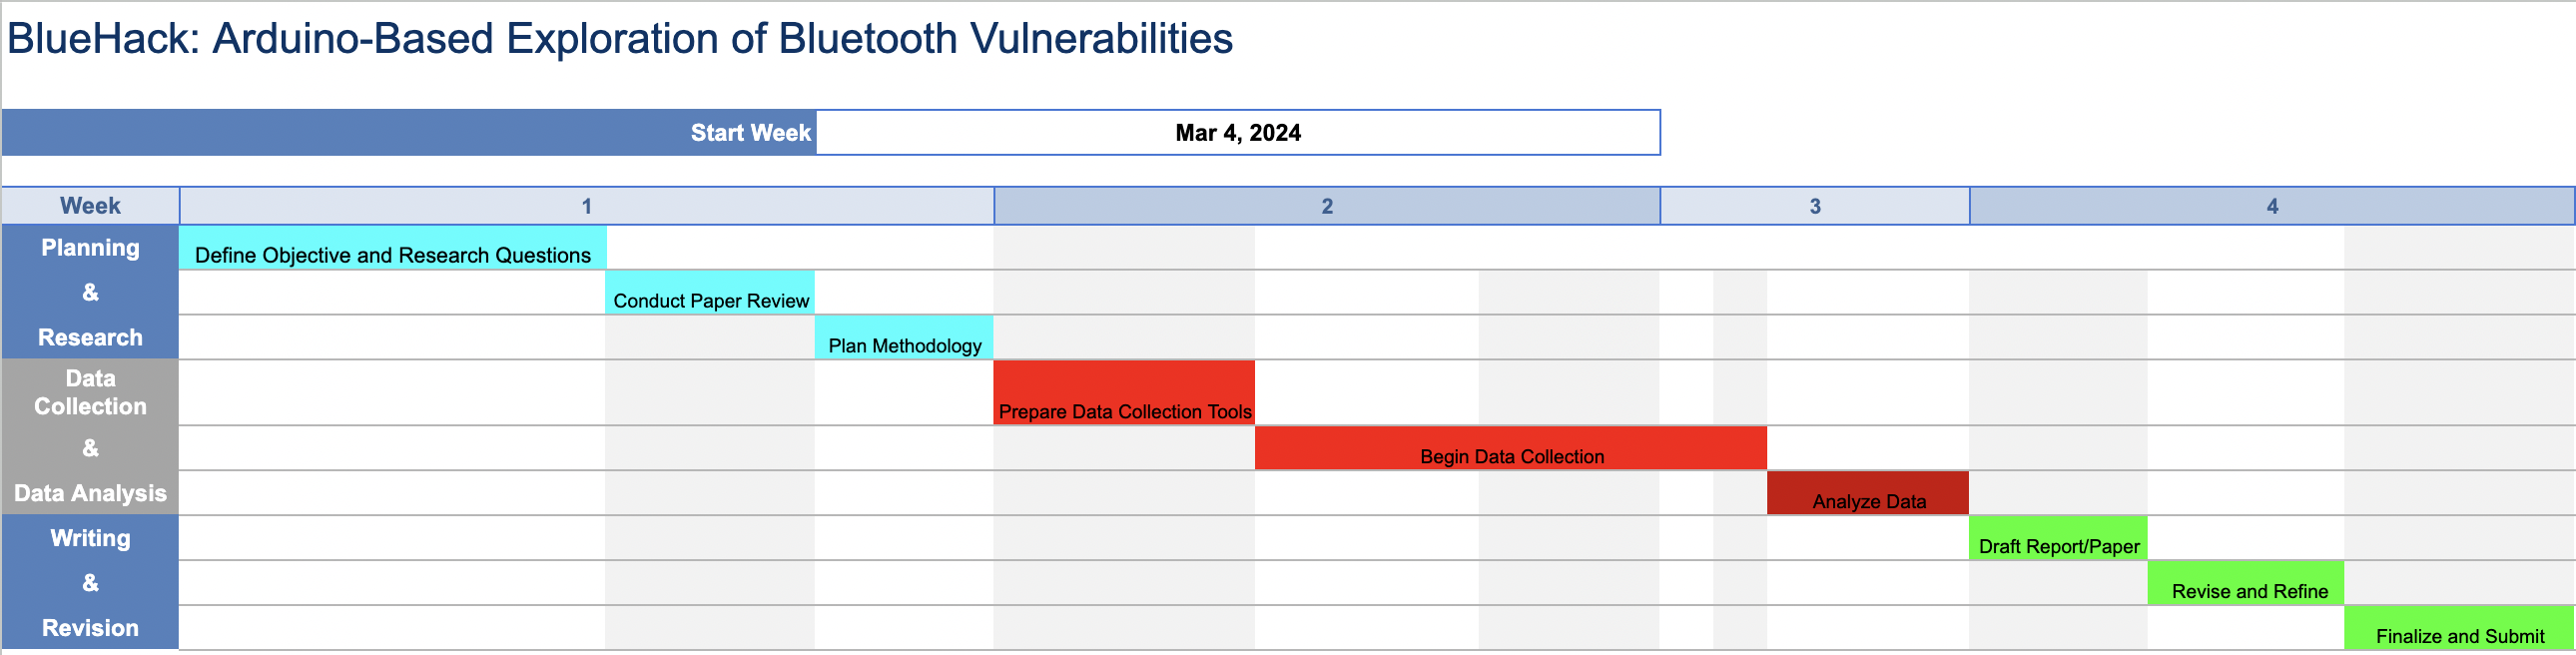
\includegraphics[width=12cm,height=30cm,keepaspectratio]{Project_Timeline.png}
    \caption{Weekly Project Timeline Over A One Month Period}
\end{figure}

    The image identifies the Project timeline. The first week is dedicated to planning and research, which includes defining objectives and research questions, conducting a paper review, and planning methodology. In the second week, the focus shifts to preparing data collection tools and beginning the actual data collection. The third week is centered around continuing the data collection and analyzing the gathered data. The fourth and final week is reserved for drafting the report or paper, revising and refining the draft, and ultimately finalizing the document and submitting it.

    

    \begin{figure}[htp]
    \centering
    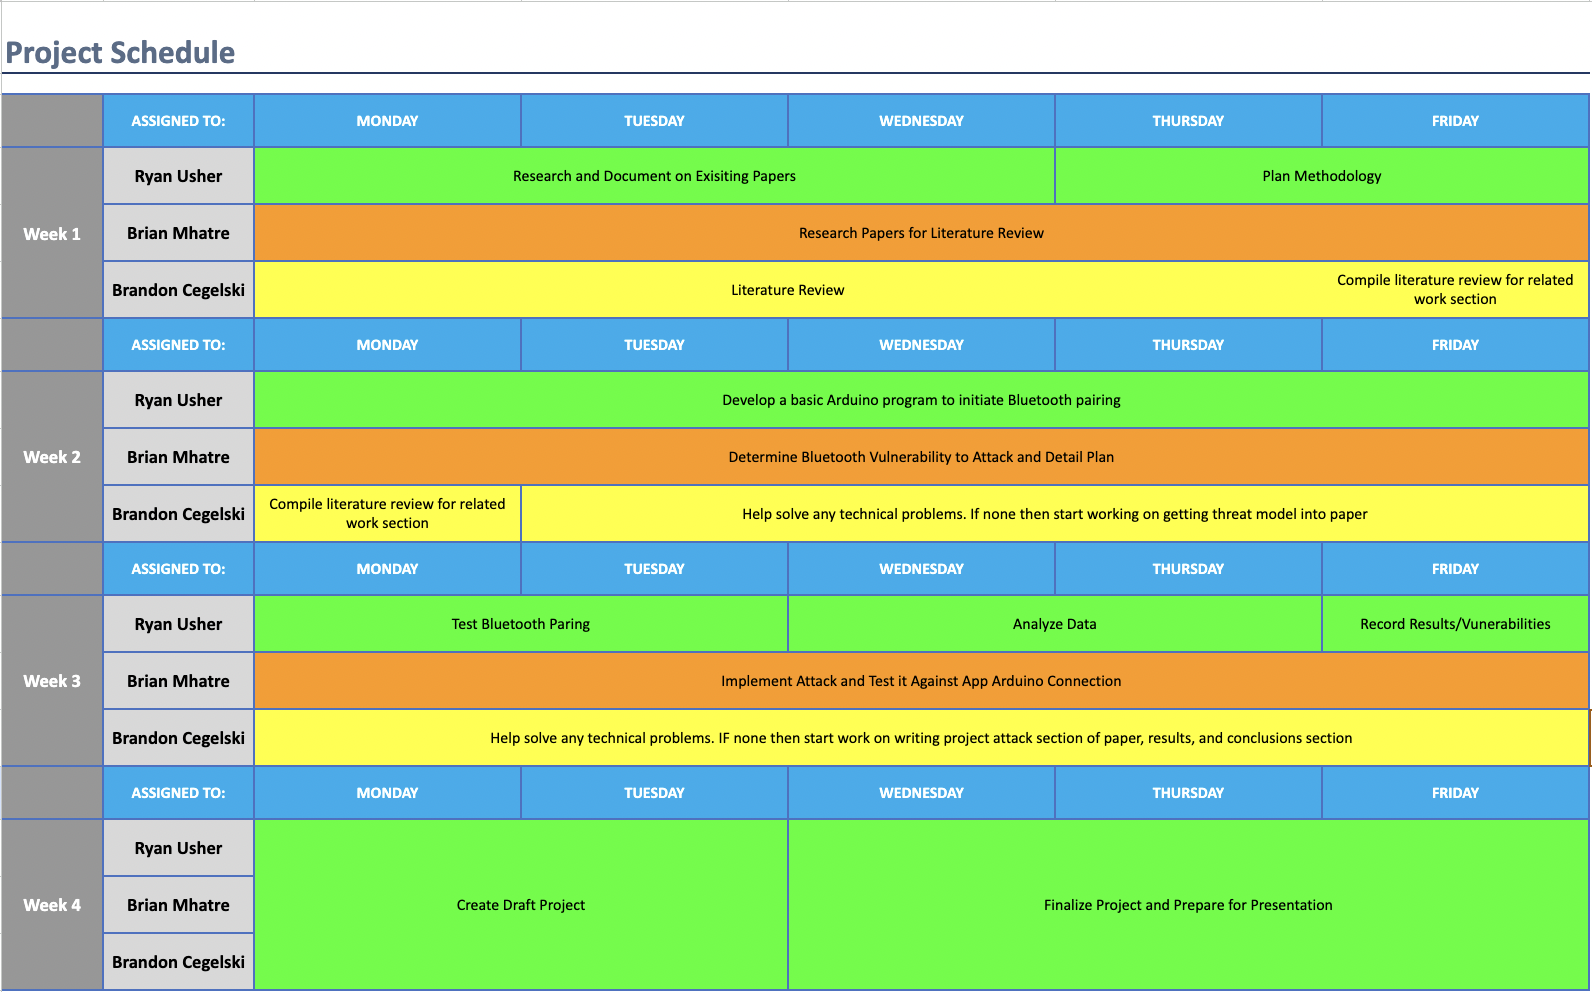
\includegraphics[width=12cm,height=30cm,keepaspectratio]{IndividualTimeline.png}
    \caption{Individual Project Timeline Over A One Month Period}
\end{figure}


    \section{Team Member Roles}

Ryan Usher: Project Lead
\begin{itemize}
    \item Oversee project kickoff and ensure team alignment with project objectives
    \item Manage the setup for data collection tools and resources.
    \item Ensure the methods are correctly applied.

\end{itemize}

Brian Mhatre: Research Analyst
\begin{itemize}
    \item Find papers and write summaries for literature review.
    \item Implment man in the middle attack for BLE.
    \item Test implmentation and collect data on the attacks effectiveness.
\end{itemize}

Brandon Cegelski: Technical Specialist
\begin{itemize}
    \item ...
    \item ...
    \item ...
\end{itemize}


\end{document}
